\documentclass[dvipdfmx]{jsarticle}

\title{ブロック落しゲーム(JavaScript)}
\author{Seiichi Nukayama}
\date{2020-06-21}
\usepackage{tcolorbox}
\usepackage{color}
\usepackage{listings, plistings}

% Java
\lstset{% 
  frame=single,
  backgroundcolor={\color[gray]{.9}},
  stringstyle={\ttfamily \color[rgb]{0,0,1}},
  commentstyle={\itshape \color[cmyk]{1,0,1,0}},
  identifierstyle={\ttfamily}, 
  keywordstyle={\ttfamily \color[cmyk]{0,1,0,0}},
  basicstyle={\ttfamily},
  breaklines=true,
  xleftmargin=0zw,
  xrightmargin=0zw,
  framerule=.2pt,
  columns=[l]{fullflexible},
  numbers=left,
  stepnumber=1,
  numberstyle={\scriptsize},
  numbersep=1em,
  language={Java},
  lineskip=-0.5zw,
  morecomment={[s][{\color[cmyk]{1,0,0,0}}]{/**}{*/}},
}
%\usepackage[dvipdfmx]{graphicx}
\usepackage{url}
\usepackage[dvipdfmx]{hyperref}
\usepackage{amsmath, amssymb}
\usepackage{itembkbx}
\usepackage{eclbkbox}	% required for `\breakbox' (yatex added)
\usepackage{setspace}
\usepackage{multicol}
\fboxrule=1pt
\parindent=1em
\begin{document}

%% 修正時刻: Sun Jun 21 08:35:35 2020


\section{落下物を描く}

program.js に 以下のように gamekaishi()関数を追加します。

\begin{lstlisting}
 function gamekaishi() {
    // Canvasを取得
    const gamegamen = document.getElementById('game');

    const cg =gamegamen.getContext('2d');

	let x = 4;
	let y = 0;

	cg.fillStyle = '#cc00cc';
	cg.strokeStyle = '#aaaaaa';

	cg.fillRect(x * 20, y, 20, 20);
	cg.strokeRect(x * 20, y, 20, 20);

	cg.fillRect((x + 1) * 20, y, 20, 20);
	cg.strokeRect((x + 1) * 20, y, 20, 20);

	cg.fillRect((x + 2)   * 20, y, 20, 20);
	cg.strokeRect((x + 2) * 20, y, 20, 20);

	cg.fillRect((x  + 1) * 20, (y + 1) * 20, 20, 20);
	cg.strokeRect((x + 1) * 20, (y + 1) * 20, 20, 20);
}
\end{lstlisting}

そして、このgamekaishi()関数を以下のタグのonclick属性に指定します。

\fbox{\textless body onload=''hajime()`` onclick=''gameKaishi()``\textgreater}

\fbox{\textless button id=''kaishibtn'' onclick=''gamekaishi()``\textgreater
ゲーム\textless br\textgreater スタート\textless /button\textgreater}

``ゲームスタート''をクリックするか、画面をクリックすると、画面上部に凸型の
図形が現れます。

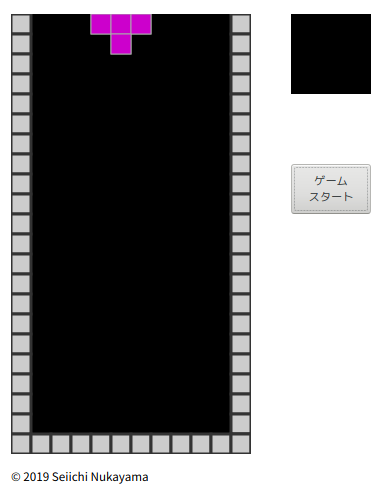
\includegraphics[width=5cm]{game3.png}

\end{document}

%% 修正時刻: Sat May  2 15:10:04 2020


%% 修正時刻: Sun Jun 21 11:46:40 2020
